\documentclass[a4paper, 12pt]{article}
%\documentclass{book}

% Important Packages:
 \usepackage{amsmath}    % need for subequations
 \usepackage{amsfonts}
 \usepackage{amsthm}
 \usepackage{graphicx}   % need for figures
 \usepackage{verbatim}   % useful for program listings
 %\usepackage{subfig}  % use for side-by-side figures
 %\usepackage{wrapfig}
 %\usepackage{listings}	 % creates code blocks
 %\usepackage[colorlinks=true]{hyperref}   % use for hypertext links, including
                     % those to external documents and URLs
 %\usepackage{multirow}
 %\usepackage{tikz}
 %\usepackage{enumerate}
 %\usetikzlibrary{decorations.pathreplacing,decorations.pathmorphing}
 %\usetikzlibrary{calc}
 %\usepackage[colorinlistoftodos]{todonotes}
 \usepackage{tikz,tkz-euclide}
 
 \usetikzlibrary{calc,patterns,angles,quotes}
\usetkzobj{all}

\def\deg{^{\circ}}
\newcommand\heading[1]{\ \\\large{\textbf{#1}}}
\newcommand\ora[1]{\overrightarrow{#1}}

%------------------end---preamble--------------------
 
 % Useful macros 
 \def\tcb#1{\color{blue}{#1}}
 \def\tcr#1{\color{red}{#1}}	
 \def\tcg#1{\color{green}{#1}}
 \def\be{\begin{eqnarray}}	 	\def\ee{\end{eqnarray}}
 \def\bea{\begin{eqnarray}}	 	\def\eea{\end{eqnarray}}
 \def\bean{\begin{eqnarray*}}	\def\eean{\end{eqnarray*}}
 
 \def\D{\displaystyle}
 \def\T{\textstyle}
 \def\l{\left}
 \def\r{\right}
 \def\nf{n_{\!f}} % quark flavours
 \def\pa{\partial}
 \def\eg{e.\,g.}
 \def\ie{i.\,e.}

 \def\be{\begin{equation}}
 \def\ee{\end{equation}}
 \def\bea{\begin{eqnarray}}
 \def\eea{\end{eqnarray}}
 \def\bean{\begin{eqnarray*}}
 \def\eean{\end{eqnarray*}}
 \def\gsim{\mathrel{\rlap{\lower0.2em\hbox{$\sim$}}\raise0.2em\hbox{$>$}}}
 \def\ksim{\mathrel{\rlap{\lower0.2em\hbox{$\sim$}}\raise0.2em\hbox{$<$}}}
 \def\kg{\mathrel{\rlap{\lower0.25em\hbox{$>$}}\raise0.25em\hbox{$<$}}}
 
 \def\AA{${\buildrel_{\circ} \over {\mathrm{A}}}$}
 \def\bm#1{\mbox{\boldmath$#1$}}
 \newcommand{\eq}[1]{(\ref{#1})} 
 \def\pd{\partial}
 \def\d{\textrm{d}} 
 \def\T{\textstyle}
 \def\eg{e.\,g.}	% exempli gratia (for the sake of example)
 \def\ie{i.\,e.}	% id est (that is)


 % Page configuration:
 \topmargin -2.0cm
 \oddsidemargin -0.85cm
 \evensidemargin -0.85cm
 \textwidth 18cm
 \textheight 24cm
 
\begin{document}
\begin{center}
\textbf{Stellenbosch Camp December 2018 \\ Senior Test 1} \\
\textbf{Solutions}
\end{center}
\vspace{5mm}

\begin{enumerate}
    % EGMO 2013 solutions: https://www.egmo.org/egmos/egmo2/solutions.pdf

    % QUESTION 1
    \item[1.] Let $d = \textrm{gcd}(m, n)$, and denote $m = da$ and $n = db$ where $a, b$ are two positive integers. We note that $\textrm{lcm}(m, n) = mn/d$. Since $a, b \geq 1$, we note
    \begin{align*}
        (a-1)(b-1) &\geq 0 \\
        \iff \quad \hspace{4.2mm} a + b &\leq 1 + ab \\
        \iff \quad da + db &\leq d + dab \\
        \iff \quad \hspace{2mm} m + n &\leq \textrm{gcd}(m, n) + \textrm{lcm}(m, n) 
    \end{align*}
    which proves the problem statement. Note that equality occurs only if either $a = 1$ or $b = 1$, which occurs iff $m$ divides $n$ or $n$ divides $m$. \qed \\
    \vspace{5mm}
    
    % QUESTION 2
    \item[2.] We first prove injectivity. That is, if $f(a) = f(b)$ for some $a, b \in \mathbb{R}$, then $a = b$. We have
    \begin{align*}
        f(a) &= f(b) \\
        \implies \quad f(f(a + 0)) &= f(f(b + 0)) \\
        \implies \quad \hspace{5.5mm} a + f(0) &= b + f(0) \\
        \implies \quad \hspace{18mm} a &= b 
    \end{align*}
    thus proving injectivity. Now substituting $y = 0$ yields $f(f(x)) = f(x)$, which, by injectivity, implies $f(x) = x$ as the only solution. One easily checks that this solution satisfies the functional equation. \qed \\
    \vspace{5mm}
    
    % QUESTION 3
    \item[3.] Let $E$ and $F$ be the feet of the perpendiculars from $B$ and $C$ respectively.\\
	Note, since $AB$ and $AC$ are diameters, the angles $\angle BNA=\angle CPA=90\deg$. Since we have $\angle NFA=\angle AEP=90\deg$, we get that $AN$ is tangent to the circumcircle of $\triangle NFB$, and $AP$ is tangent to the circumcircle of $\triangle PEC$. Lastly, we know that $BFEC$ is a cyclic quadrilateral. So by using power of a point in the circles $NFB$, $PEC$, and $BFEC$, we obtain
	\begin{flalign}
		&&AN^2&=BA \cdot AF= CA \cdot AE =AP^2 &\nonumber \\
		&\therefore& AN&=AP&\nonumber	
	\end{flalign}
	But we already have, $AN=AM$, and $AP=AQ$. Thus, $AN=AM=AP=AQ$. So $M$, $N$, $P$, and $Q$ are all equidistant from $A$, and thus lie on a common circle centred at $A$. \qed

    \begin{figure}[h]
	\begin{center}
	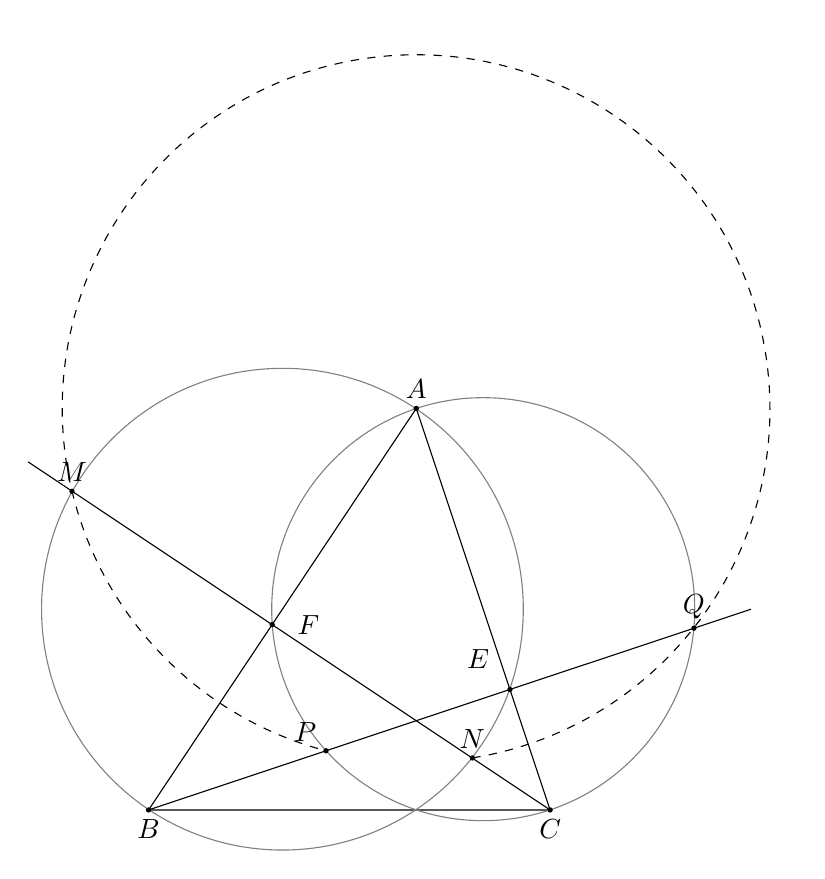
\begin{tikzpicture}[scale=1.7]
		% \useasboundingbox (-2,-2) rectangle  (2,2);
		\coordinate (B) at (-2,-1);
		\coordinate (A) at (0,2);
		\coordinate (C) at (1,-1);
		\tkzDefLine[orthogonal=through C](B,A) \tkzGetPoint{h1};
		\tkzDefLine[orthogonal=through B](C,A) \tkzGetPoint{h2};
		\draw[-] (A)--(B)--(C)--(A);
		\tkzDrawLine[thin,add=0 and 0.3](C,h1);
		\tkzDrawLine[thin,add=1.5 and -1](B,h2);
		\coordinate (m1) at (-1,0.5);
		\coordinate (m2) at (0.5,0.5);
		\tkzDrawCircle[thin](m1,A);
		\tkzDrawCircle[thin](m2,A);
		\tkzInterLC(C,h1)(m1,A)\tkzGetPoints{M}{N};
		\tkzInterLC(B,h2)(m2,A)\tkzGetPoints{P}{Q};
		\tkzInterLL(C,h1)(A,B)\tkzGetPoint{F};
		\tkzInterLL(B,h2)(A,C)\tkzGetPoint{E};
		\node at (A) [above]{$A$};
		\node at (B) [below]{$B$};
		\node at (C) [below]{$C$};
		\node at (E) [above left=0.2]{$E$};
		\node at (F) [right=0.2]{$F$};
		\node at (M) [above]{$M$};
		\node at (N) [above]{$N$};
		\node at (P) [above left]{$P$};
		\node at (Q) [above]{$Q$};
		\tkzDefCircle[circum](M,N,P)\tkzGetPoint{O};
		\tkzDrawArc[thin,dashed](O,N)(P);
		\fill[color=black!100] (A) circle (0.02) ;
		\fill[color=black!100] (B) circle (0.02) ;
		\fill[color=black!100] (C) circle (0.02) ;
		\fill[color=black!100] (E) circle (0.02) ;
		\fill[color=black!100] (F) circle (0.02) ;
		\fill[color=black!100] (M) circle (0.02) ;
		\fill[color=black!100] (N) circle (0.02) ;
		\fill[color=black!100] (P) circle (0.02) ;
		\fill[color=black!100] (Q) circle (0.02) ;
		\end{tikzpicture}
	\end{center}		
	\end{figure}
    
    
    \newpage
    % QUESTION 4
    \item[4.]  Define a subset $U$ of $S_n$ as \textit{unbalanced} if it is not balanced. We define a map $f : P(S_n) \to P(S_n)$ from subsets of $S_n$ to subsets of $S_n$. Let $U \in P(S_n)$ be a subset of $S_n$ and define $f(U)$ as the subset  $\{ n -k+1 \;:\; k \in U  \}$ (i.e. it's a reversal map sending each element $k$ in $U$ to $n-k+1$). Note that we clearly have $f(f(U)) = U$ for all $U \in P(S_n)$. Furthermore, we easily note that the map flips the relative order of the mean and median of $U$ (i.e. if $U_\textrm{mean} < U_\textrm{median}$ then $f(U)_\textrm{mean} > f(U)_\textrm{median}$). Thus, if $U$ is unbalanced, then $f(U) \not = U$.

    Therefore, we have paired up each unbalanced set uniquely with another unbalanced set, proving that there are an \textit{even} number of unbalanced sets. As the total number of non-empty subsets is $2^n-1$, there are thus an \textit{odd} number of balanced subsets. \qed \\
    \vspace{5mm}
    
    % QUESTION 5
    \item[5.]  Let $n = 15$. Note that the set $\{1, 2^2, 3^2, 5^2, 7^2, \dots, 43^2 \}$ consisting of 1 and the squares of the first 14 primes is a pairwise coprime set not containing any prime. Thus, if $n$ satisfies the problem condition, then $n \geq 16$.  We now prove that amongst any 16 pairwise coprime elements, at least one is prime. 

    Let $A = \{a_1, a_2, \dots, a_n\}$ be a set with $n \geq 16$ pairwise coprime elements, and order it in order of smallest prime dividing each element (if 1 is included, let $a_1 = 1$). Let $p_i$ be the smallest prime dividing $a_i$. As $A$ is pairwise coprime, we have $p_2 < p_3 < p_4 < \dots < p_n$. Thus, as $p_2 \geq 2$, we have $p_n \geq 47$ as 47 is the 15th smallest prime. Now assuming that $a_n$ is not prime, we have $a_n \geq p_n^2 \geq 2209 > 2018$ which yields a contradiction. Thus $a_n$ is prime, which proves $n = 16$ is the minimal $n$ satisfying the problem condition. \qed

    

\end{enumerate}
\end{document}




